\documentclass[a4paper]{article}

\pdfmajorversion=1
\pdfminorversion=7
\pdfcompresslevel=9
\pdfobjcompresslevel=2

\usepackage[hidelinks]{hyperref}
\usepackage[margin=60pt]{geometry}
\usepackage[utf8]{inputenc}
\usepackage[english]{babel}
\usepackage{amsmath}
\usepackage{amssymb}
\usepackage{colortbl}
\usepackage{graphicx}
\usepackage{mathtools}
\usepackage{subcaption}
\usepackage{tabularx}
\usepackage{xcolor}

\setlength{\parindent}{0pt}

\hypersetup{
    pdftitle={Formal Digital Twin of a LEGO® MINDSTROMS™ Production Plant},
    pdfauthor={Andrea Infantino, Riccardo Motta, Matteo Negro}
}

\captionsetup[figure]{labelfont=bf}

\newcommand{\figureref}[1]{\textsf{\hyperref[#1]{Figure \ref*{#1}}}}
\newcommand{\sectionref}[1]{\textsf{\hyperref[#1]{Section \ref*{#1}: \nameref*{#1} (page \pageref*{#1})}}}
\newcommand{\propertyref}[2]{\textsf{\hyperref[#2]{Property #1: \nameref*{#2}}}}
\newcommand{\nbvspace}[1][3]{\vspace*{\stretch{#1}}}

\newcommand{\formulacomment}[2]{\underset{\varphi_{#1}}{\underbrace{#2}}}
\newcommand{\formulatext}[1]{\text{\texttt{#1}}}

\newcommand{\parametertt}{\fontfamily{lmtt}\fontseries{b}\selectfont}
\newcommand{\parametertitle}[2]{\multicolumn{#1}{|c|}{#2}}
\newcommand{\parametercontent}[2]{\multicolumn{#1}{|c|}{#2}}

\renewcommand\tabularxcolumn[1]{m{#1}}

\arrayrulecolor{lightgray}

\begin{document}

    \begin{titlepage}

        \begin{center}

            \nbvspace[1]

            
\includegraphics[width=0.3\columnwidth]{./images/polimi}

            \nbvspace[2]

            {\huge \textbf{\textsc{Formal Digital Twin of a \\ LEGO\textsuperscript{\textregistered} MINDSTROMS\texttrademark \\\medskip Production Plant}}} \\
            [3em]
            {\Large Formal Methods for Concurrent and Real-Time Systems} \\
            [1.5em]
            {\Large A.Y. 2022-2023}

            \nbvspace[8]

            \begin{tabular}{lrp{0.04\columnwidth}lrp{0.04\columnwidth}lr}
                \multicolumn{2}{c}{\large \textbf{Andrea Infantino}} & & \multicolumn{2}{c}{\large \textbf{Riccardo Motta}} & & \multicolumn{2}{c}{\large \textbf{Matteo Negro}} \\
                Person ID & 10671720 & & Person ID & 10658639 & & Person ID & 10642961 \\
                Student ID & 225757 & & Student ID & 218685 & & Student ID & 222025
            \end{tabular}

            \nbvspace[1]

        \end{center}

    \end{titlepage}

    \tableofcontents{}

    \pagebreak

    \section{Model Description}

    This section provides a description of the production plant with some implementation details, together with all the components that make it up. The motivations behind these modelling choices can be found in \sectionref{section:design_decisions}.

    \subsection{The Production Plant}

    \begin{figure}[h!]
        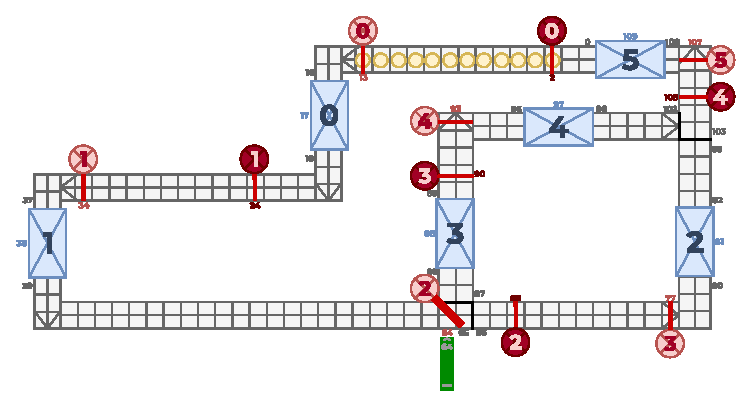
\includegraphics[width=\columnwidth]{./images/plant}
        \caption{the production plant we modelled.}
        \label{figure:scheme}
    \end{figure}

    This is the plant we modelled in our project. The yellow circles are the workpieces, the blue rectangles are the processing stations, the light and dark red circles are the sensors and the green bar is the flow controller.

    \paragraph{Notes on the scheme} In order to make the entire description of our project as much clear as posssible, we enhanced the original scheme with the IDs we assigned to stations and laser sensors, and with the positions of the slots that compose the conveyor belt. Note that we decided to consider the stations as particular components placed above a normal slot; therefore we have two numbers defining each station: one refers to the position of the slot, while the other the ID of the station.

    \subsection{General Overview}

    The model of our system is made of 6 different components which interact between them to coordinate the entire production plant. Some of them are also instantiated many times in order to have a simpler modelling of the entire system.

    \paragraph{Initializer} It's a fictitious component which represents the entry point of the whole system. It allows us to instantiate all the workpieces in the correct positions of the conveyor belt (positions which start from position 13 and ends in position 2 in our model) and works as the general clock of the system.

    \paragraph{Motor} This is the real motor of the system. According to the speed at which the conveyor belt should be moving, uses the clock to make all the workpieces move and synchronizes the whole system.

    \paragraph{Conveyor belt} It's the manager of the conveyor belt, in charge of moving around all the workpieces. In our model it's also the one in charge of preventing workpieces from entering a station, based on the information gathered by the laser sensors. Finally, it handles the positions where the two branches of the plant start and merge.

    \paragraph{Processing stations} They are the ones in charge of processing the various workpieces, once they get into them. We implemented a single template for them, which is instantiated as many times as needed in order to recreate the plant. As already explained, each station is assumed to be placed above a slot of the conveyor belt.

    \paragraph{Laser sensors} We have modelled them in two different ways according to their functionalities. The ones guarding the entrance of a station are called \texttt{InSensor} (represented as light red circles in \figureref{figure:scheme}), while the ones guarding the queue and preventing the station right before it to release a workpiece are called \texttt{OutSensor} (represented as dark red circles). Like the stations, they are represented as a single template (one for each type), instantiated multiple times.

    \paragraph{Flow controller} This is the green piece of \figureref{figure:scheme}. It is pre-configured with a specific policy (which is customizable) and decides where to send the workpieces once they get at position 65 of the conveyor belt. The available policies are the following ones:
    \begin{enumerate}
        \item[0.] Sends the workpieces on the alternative branch until its queue is full, otherwise lets the workpieces proceed on the main branch;
        \item[1.] Lets all the workpieces to flow on the main branch;
        \item[2.] Sends all the workpieces on the alternative branch;
        \item[3.] Every time a workpiece is in front of him sends it on a different path with respect to the one taken by the previous workpiece.
    \end{enumerate}

    \subsection{Initializer (\texttt{Initializer})}

    The initializer is the fundamental entry point of our whole system; it is a meta component that performs two different actions.

    \paragraph{Initialization} Initializes the system by placing the workpieces starting from the slot guarded by the first \texttt{InSensor} (index 0), and continuing backward with an upper limit of 12 workpieces.

    \paragraph{Global synchronization} In order to have a simpler model to verify, we decided to have a unique clock for the whole system. This TA performs as the general clock on which all the components of our plant, directly or indirectly synchronize (usually by means of the signals generated by the motor).

    \subsection{Motor (\texttt{Motor})}

    As the name says, this is the meta component that manages all the signals used by the sensors, the conveyor belt and the stations, to synchronize the movement of the workpieces. The two signals which it generates are presented here.

    \paragraph{Conveyor belt's tick (\texttt{tick\_belt}, also used by the stations)} It's the signal which makes the conveyor belt move all the workpieces it can one step forward (taking into account also the branch in the conveyor belt).

    \paragraph{Laser sensors and stations' tick (\texttt{tick\_sensor})} In order to avoid any potential race condition, we decided to send a signal right before \texttt{tick\_belt}. This allows us to update the state of the laser sensors (i.e., check whether there is a workpiece right below them or not) and to perform some state-changing actions on all the stations (if needed).

    \subsection{Conveyor Belt (\texttt{ConveyorBelt})}

    It's the entity which handles the plant's conveyor belt. It's a small automaton since all the underlying complexity of the conveyor belt's management is hidden behind the \texttt{update()} function. This is the most complex component of our plant since manages a lot of different things.

    \paragraph{Workpieces position} Any workpiece on a non-critical position (which is any in the following situations) is moved ahead of one slot every time the \texttt{update()} function is called.

    \paragraph{Stations and sensors management} Once a workpiece passes the \texttt{InSensor} of a station, it blocks any other workpiece wanting to proceed to the station itself until the sensor tells that the station is free and a new workpiece can flow again towards it.

    \paragraph{Queue management} Every time a workpiece is blocked in a specific location and some other one wants to proceed, the conveyor belt blocks it until the first one is free to move again. Since we are scanning the belt from the last positions backward this situation is easily managed since we can't place a workpiece on top of another one.

    \paragraph{Conveyor belt branch and merge} In order to be updated about which branch the next workpiece should take, we decided to keep the Conveyor Belt always ready to receive the signal \texttt{switch\_branch?}. This allows us to directly use the \texttt{update()} function to move the workpieces on the correct branch. Also, the merge of the two branches is (easily) managed by the conveyor belt, since, by scanning it backward, once we move a piece in the merge position of the belt (position 103), no other one can be put in the same place, thus, blocking it from proceeding, which is exactly what happens in reality.

    \subsection{Processing stations (\texttt{Station})}

    \begin{figure}[h!]
        \centering
        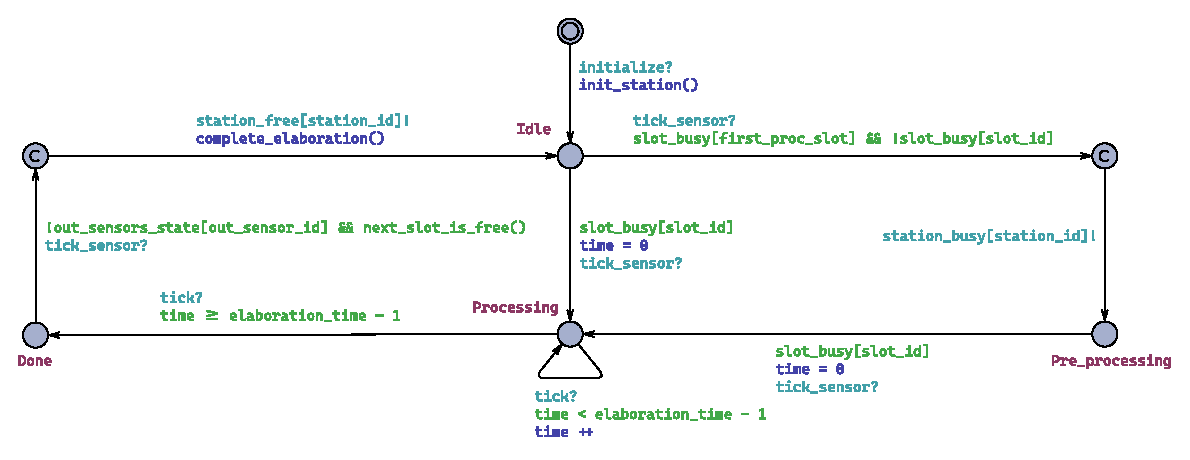
\includegraphics[width=\columnwidth]{./images/automata/station}
        \caption{the Timed Automata of every station.}
    \end{figure}

    The stations model the various processes the workpieces need to go through during production. The automaton is divided in four different main states, each one representing a status in which the station can be.

    \paragraph{Idle} This is the main state of the station, in which it doesn't have to perform any action but to wait for a workpiece to be ready for the processing.

    \paragraph{Preprocessing} When the laser sensors which is guarding the entrance of the station signals that a workpiece is approaching to it, the station moves to this state waiting for the entrance of the workpiece.

    \paragraph{Processing} Once the workpiece is entered, the station starts processing it. In the model, the automaton isn't performing any real task on the workpiece, but it's simply waiting for its processing time to pass. In order to improve verification performance, we discretized the time, and so we use a counter synchronized with the global clock in order to model the time passing.

    \paragraph{Done} Once the processing time is elapsed, the station moves to this state, where it waits for the right time to release the workpiece on the conveyor belt. It synchronizes with the conveyor belt itself and with the sensors guarding the queue of the following station, in order to know if the workpiece can be release or has to be held inside the station itself. Once the workpiece is released, the station returns to its \textit{idle} state, waiting for the next processing cycle.

    \subsection{Processing station's input guard (\texttt{InSensor})}

    These are the laser sensors that guard the entrance of a specific station. If a workpiece oversteps it, the laser sensor is equipped with a physical barrier which blocks any other following workpiece from proceeding towards the guarded station, until it is free again.

    \subsection{Queue's guard (\texttt{OutSensor})}

    Right before a station there is always an \texttt{InSensor} which guards its entrance, but  it can be preceded by another sensor, which guards the queue. Once the station's guard blocks a workpiece, others may arrive forming a queue of workpieces. This queue may have a maximum length. If the queue reaches its maximum, the sensor prevents the preceding station to release a workpiece until the queue is no longer full.

    \subsection{Flow controller (\texttt{FlowController\_*})}

    \begin{figure}[h!]
        \centering
        \begin{tabularx}{\linewidth}{*{2}{>{\centering\arraybackslash}X}}
            \begin{subfigure}{\linewidth}
                \caption{Controller v0}
            \end{subfigure} &
            \begin{subfigure}{\linewidth}
                \caption{Controller v1}
            \end{subfigure} \\
            \begin{subfigure}{0.5\columnwidth}
                \centering
                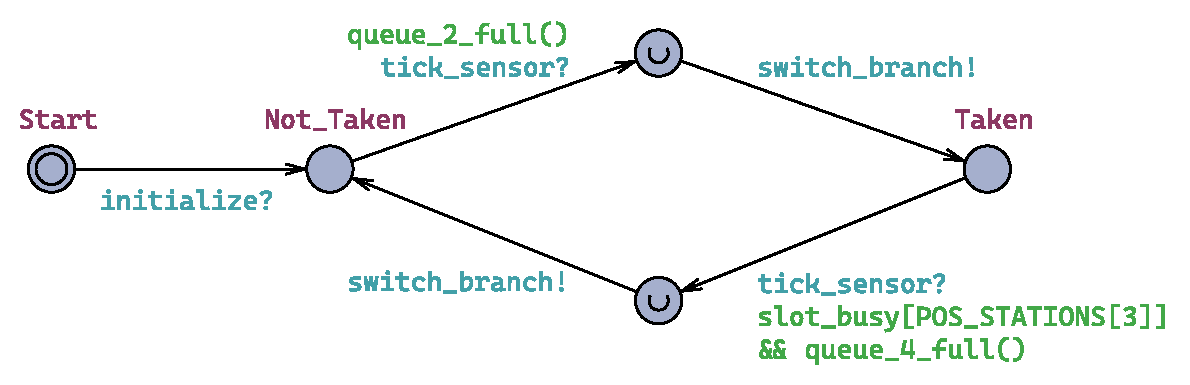
\includegraphics[width=\columnwidth]{images/automata/flow_controller_0}
            \end{subfigure} &
            \begin{subfigure}{0.23\columnwidth}  
                \centering
                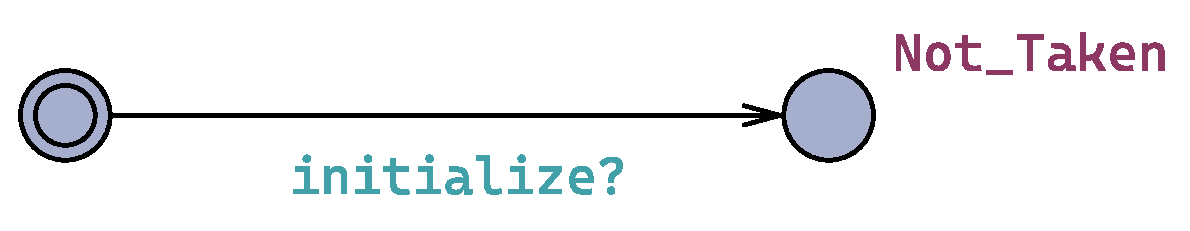
\includegraphics[width=\columnwidth]{images/automata/flow_controller_1}
            \end{subfigure} \\
            \begin{subfigure}{0.27\columnwidth}   
                \centering 
                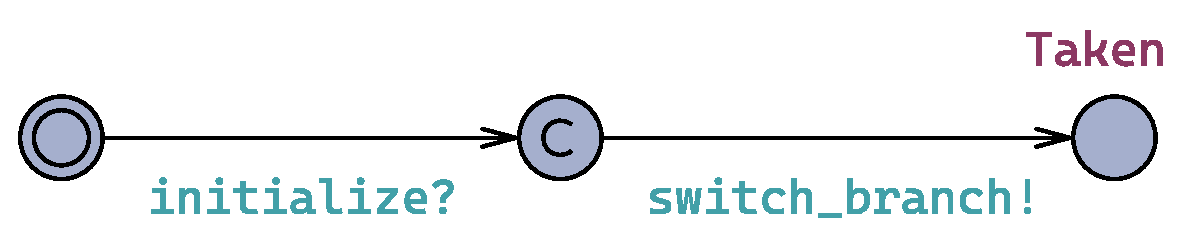
\includegraphics[width=\textwidth]{images/automata/flow_controller_2}
            \end{subfigure} &
            \begin{subfigure}{0.45\columnwidth}   
                \centering 
                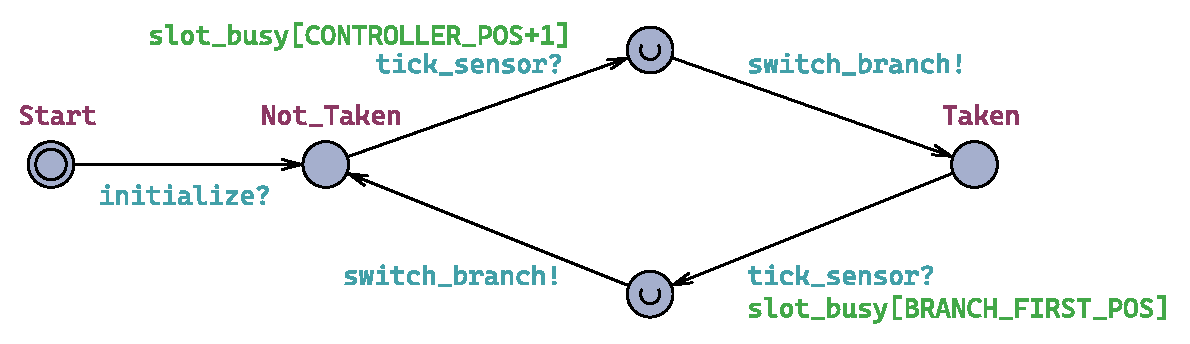
\includegraphics[width=\columnwidth]{images/automata/flow_controller_3}
            \end{subfigure} \\
            \begin{subfigure}{\linewidth}
                \caption{Controller v2}
            \end{subfigure} &
            \begin{subfigure}{\linewidth}
                \caption{Controller v3}
            \end{subfigure}
        \end{tabularx}
        \caption{the Timed Automata of the various types of controllers.}
    \end{figure}

    As explained in the introduction, these are the various policy schedules we implemented. Each one of them represents a different way to schedule the workpieces on the processing stations. Starting from the easiest ones, the ones in which all the workpieces follow the same path (either the direct one or the alternative one), to more complex ones, like the one in which we keep track of the queues in front of the first stations of the branch.\medskip

    Since the effective movement of the various workpieces is managed by the conveyor belt, these automata send a signal (\texttt{switch\_branch}) to it each time the path followed by the workpieces has to be changed.
    
    \section{Design Decisions} \label{section:design_decisions}

    \subsection{Hypothesis}

    \paragraph{Slots' numbering} We numbered the slots as shown in \figureref{figure:scheme}. This helped us in the management of the conveyor belt's update function and implicitly allowed us to solve the problem of merging the two alternative paths at position 103. In the (possible) corner case in which both position 85 and position 102 are carrying a workpiece at the same time (i.e., they are simultaneously trying to place a workpiece on slot 103), we decided to apply the following policy: the first piece to flow is always the one coming from station 4. This is, of course, a simplification. A more complicated approach could have been taken, like randomly picking one of the two workpieces, but we decided to keep it as simple as we could.

    \paragraph{Maximum number of circulating workpieces} We decided to stick with the representation of \figureref{figure:scheme}. So we have at most twelve workpieces circulating in the production plant, and they all are initially placed from position 13, proceeding backward. Please, notice that if the number of workpieces exceeds the position of the first \texttt{OutSensor} (which can be changed by project hypothesis), one of the properties isn't verified. However, this is normal since during the initialization of the plant we are already exceeding the maximum queue's length of the first one.

    \paragraph{Time discretization} This will be more clear in the next part, where we describe the main optimization steps we did, but, in brief, we discretized the time in order to have a better synchronization mechanism of the whole plant.

    \subsection{Optimizations}

    Here we present all the main optimization steps we performed in order to have the final model.

    \subsubsection{The basic idea}

    \paragraph{Idea} At first, we decided to model every single entity of the plant. We had the template for generating all the single slots of the conveyor belt. This has been done in order to have a precise (and discrete) representation of the plant pointing out all the atomic components that we have.

    \paragraph{Situation} Proceeding in this way, we experienced huge verification times, due to the high number of entities and states that the software had to process each time.

    \subsubsection{Unique conveyor belt}

    \paragraph{Idea} In order to simplify the modelling of the plant and our code, we decided to group the slots of the conveyor belt all together into a single logically entity (the \texttt{ConveyorBelt}).

    \paragraph{Situation} This simplified a lot the management of all the various cases (and indeed is still present in our project), since we had a unique entity to manage the complexity derived from the movement of the various workpieces. This also works in synchronicity with the processing stations and the sensors, in order to block the pieces when needed, and with the flow controller, which communicates to the \texttt{ConveyorBelt} where to send the workpieces on the branch. By doing this we also improved significantly the verification time needed to check the properties, but we still had a huge memory consumption.

    \subsubsection{Automata simplification}

    \paragraph{Idea} Since one of the things that was making the verification process heavy and slow, was the wide number of states traversed at each iteration, we decided to try to reduce the number of total states composing the entire system at the bare minimum.

    \paragraph{Situation} We removed some superfluous states from our model, and we split the flow controller into four different ones (one for each policy), in order to instantiate only the one that we were going to use during the simulation and verification of the plant. This allowed us to have slight improvements both in verification times and memory consumption.

    \subsubsection{Unique clock}

    \paragraph{Idea} By talking with some colleagues and with the instructors we realized that we had 7 different clocks inside our project (one for the general clock of the system and one for each station); since this fact was one of the biggest bottlenecks during the verification phase, we decided to reduce them to just a general one, and to keep all the various templates synchronized with it.

    \paragraph{Situation} We added a new template, the \texttt{Motor}, which sends the right signals at the right moment to all the components that need it, while respecting the speed of the conveyor belt's movement; then we synchronized the stations' processing times with the general clock of the system (which is not related to the speed of the conveyor belt). By doing this, we reduced the number of possible transitions the system can potentially take at any instance. This allowed us to have a skyrocketing verification time, even with 12 different workpieces circulating in the production plant at the same time.

    \section{Properties}

    \subsection{No two workpieces can be in the same position at the same time} \label{property:1-2}

    Since we modelled the plant as a unique conveyor belt with the stations placed on some specific slots, this property embraces two different requirements of the production plant:
    \begin{itemize}
        \item \textit{It never happens that a station holds more than 1 workpiece};
        \item \textit{It never happens that two pieces occupy the same conveyor belt slot}.
    \end{itemize}

    Note that the slots are modelled as an array of 110 Boolean values, in which \texttt{true} corresponds to the presence of a workpiece in that position.\medskip

    In order to verify this property, we check that, after the plant has been initialized, the number of the workpieces remains constant and equal to its configured number, which can be represented in TCTL as follows:
    \[\forall \square \left(\formulacomment{1}{\formulatext{initializer.run\_state}} \implies \left(\formulacomment{2}{\sum_{i = 0}^{109} \formulatext{slot\_busy[i]}} = \formulatext{DISKS}\right)\right)\]

    \begin{itemize}
        \item \(\varphi_1\): the system has been initialized;
        \item \(\varphi_2\): the number of circulating workpieces in the production plant.
    \end{itemize}

    \subsection{Queues never exceed their maximum length} \label{property:3}

    We verified this by exploiting a custom function which, given the positions of a related pair (\texttt{InSensor}, \texttt{OutSensor}), we check that there is at least one free slot between the position of the \texttt{InSensor} and the position preceding the one of the \texttt{OutSensor}. If the property is false, it means that there is at most one extra piece in the queue. We verified this as follows:
    \[\forall \square \left(\forall i \in \left[0; 4\right] \left(\formulacomment{1}{\formulatext{outSensor(i).Locked}} \implies \formulacomment{2}{\formulatext{check\_queue(i, POS\_OUT\_SENSORS[i])}}\right)\right)\]

    \begin{itemize}
        \item \(\varphi_1\): the \(i\)-th \texttt{InSensor} is locked (the guarded station is not in \texttt{Idle});
        \item \(\varphi_2\): checks that the queue doesn't exceed its maximum length.
    \end{itemize}

    \subsection{The plant never incurs in deadlock} \label{property:4}

    In order to verify this, we checked both the automata part and the logic one. This means that we made sure to not incur in a deadlock in the transitions, and that all the pieces are continuing to circulate in the plant.\medskip

    The property for the transitions is verified with \(\forall \square \left(\neg \formulatext{deadlock}\right)\), while the second one with:
    {
        \scriptsize
        \[\forall \square \left(\neg \left(\formulacomment{1}{\left(\forall i \in \left[0; 5\right] \left(\formulatext{station(i).Processing} \vee \formulatext{station(i).Done}\right)\right)} \wedge \formulacomment{2}{\left(\forall i \in \left[0; 4\right] \formulatext{outSensor(i).Locked}\right)} \wedge \formulacomment{3}{\left(\forall i \in \left[0; 5\right] \formulatext{inSensor(i).Locked}\right)}\right)\right)\]
    }

    \begin{itemize}
        \item \(\varphi_1\): all the stations are either blocked on \texttt{Processing} or \texttt{Done};
        \item \(\varphi_2\): all the \texttt{OutSensor} are preventing pieces from exiting the stations;
        \item \(\varphi_3\): all the \texttt{InSensor} are blocking pieces from reaching the stations.
    \end{itemize}

    \section{Stochastic Version}
    
    In real world applications of abstract models, nothing is unbreakable. Every kind of concrete component can be subject to fault, errors and/or failures; that's why, in order to provide a model as much suitable to a real application context as possbile, we implemented a separate version of our original project, improved with the two following stochastic features.

    \subsection{Faulty Sensors}

    % IMAGE

    In real world, every kind of sensors might provide false positives (in our case, detection of a not actually present piece) and/or false negatives (in our case, non-detection of an actually present piece); we took into account this feature by modifying the original TA of both \texttt{InSensor} and \texttt{OutSensor} as shown in Figure 4: Starting from the original non-stochastic version of the two type of sensors, we added two couples of alternative states, \texttt{C1}-\texttt{C2} and \texttt{C3}-\texttt{C4}, respectively handling false positives and false negatives; in this way, each time the sensor is unlocked, one state among \texttt{C1} (meaning that the sensor is working properly) and \texttt{C2} (meaning that a detection error has occured) is stochastically chosen, based on a probability weight passed as parameter to the template. Similarly, every time the sensor is locked, state \texttt{C3} is visited if the sensor has performed a misreading, and state \texttt{C4} otherwise.

    \paragraph{Deadlock avoidance} As you can see in Figure 4, we added two apparently useless edges: the first from state \texttt{C1} to state \texttt{Unlocked}, and the second from state \texttt{C4} to state \texttt{Locked}; these edges are unexpectedly necessary, since they allow the sensors to check for the presence of a workpiece on the guarded slot every time the conveyor belt moves, avoinding unwanted potential deadlocks.

    \subsection{Normally distributed stations' processing times}

    The processing time of any real industrial processing station can be effectively measured in order to coordinate every other component that has to interact with it. However, even if they are usually very close one from each other, the time taken in practice is never exactly the same for every single processing; we abstracted this classical behavior by creating a normal distribution function with mean value and standard deviation passed as parameters of the \texttt{Station} template; then, each time a workpiece enters a station, the processing time needed is stochastically picked based on the computed normal distribution.

    \paragraph{UPPAAL limit} While implementing the normal distribution function, we experienced that UPPAAL is unable to compare clocks (used to keep track of the passing of the time) with \texttt{double} numbers. In order to deal with that, after have stochastically picked the needed processing time, we decided to round it to the closest integer value.

    \section{Scenarios}

    In this section we are going to propose some possible scenarios, aiming at proving the resiliency of our model both in standard and borderline situations; Furthermore, we included also some pathological cases, in which the plant fails to guarantee some properties (as it should be).

    \subsection{Scenario 1: the normality}

    This can be considered the "standard" scenario: the structure of the plant is the one depicted in the introduction. The stations' processing times have been chosen without any specific criterion, and we instructed the flow controller to equally send the workpieces on the two different branches of the conveyor belt, in the way defined above as policy number 3.

    \paragraph{Parameters} These are the parameters used to obtain \figureref{figure:scenario:1}.

    \begin{center}
        \begin{tabular}{|>{\centering\arraybackslash}p{0.14\columnwidth}|>{\centering\arraybackslash}p{0.14\columnwidth}|>{\centering\arraybackslash}p{0.14\columnwidth}|>{\centering\arraybackslash}p{0.145\columnwidth}|>{\centering\arraybackslash}p{0.3\columnwidth}|}
            \hline
            \parametertt SPEED & \parametertt DISKS & \textbf{Policy} & \parametertt \small POS\_OUT\_SENSORS & \parametertt STATIONS\_ELABORATION\_TIME \\
            \hline
            1 & 12 & 3 & {\footnotesize [2, 24, 68, 90, 105]} & [6, 7, 8, 9, 8, 7] \\
            \hline
        \end{tabular}
    \end{center}

    \begin{figure}[h!]
        \begin{subfigure}{\textwidth}
            \centering
            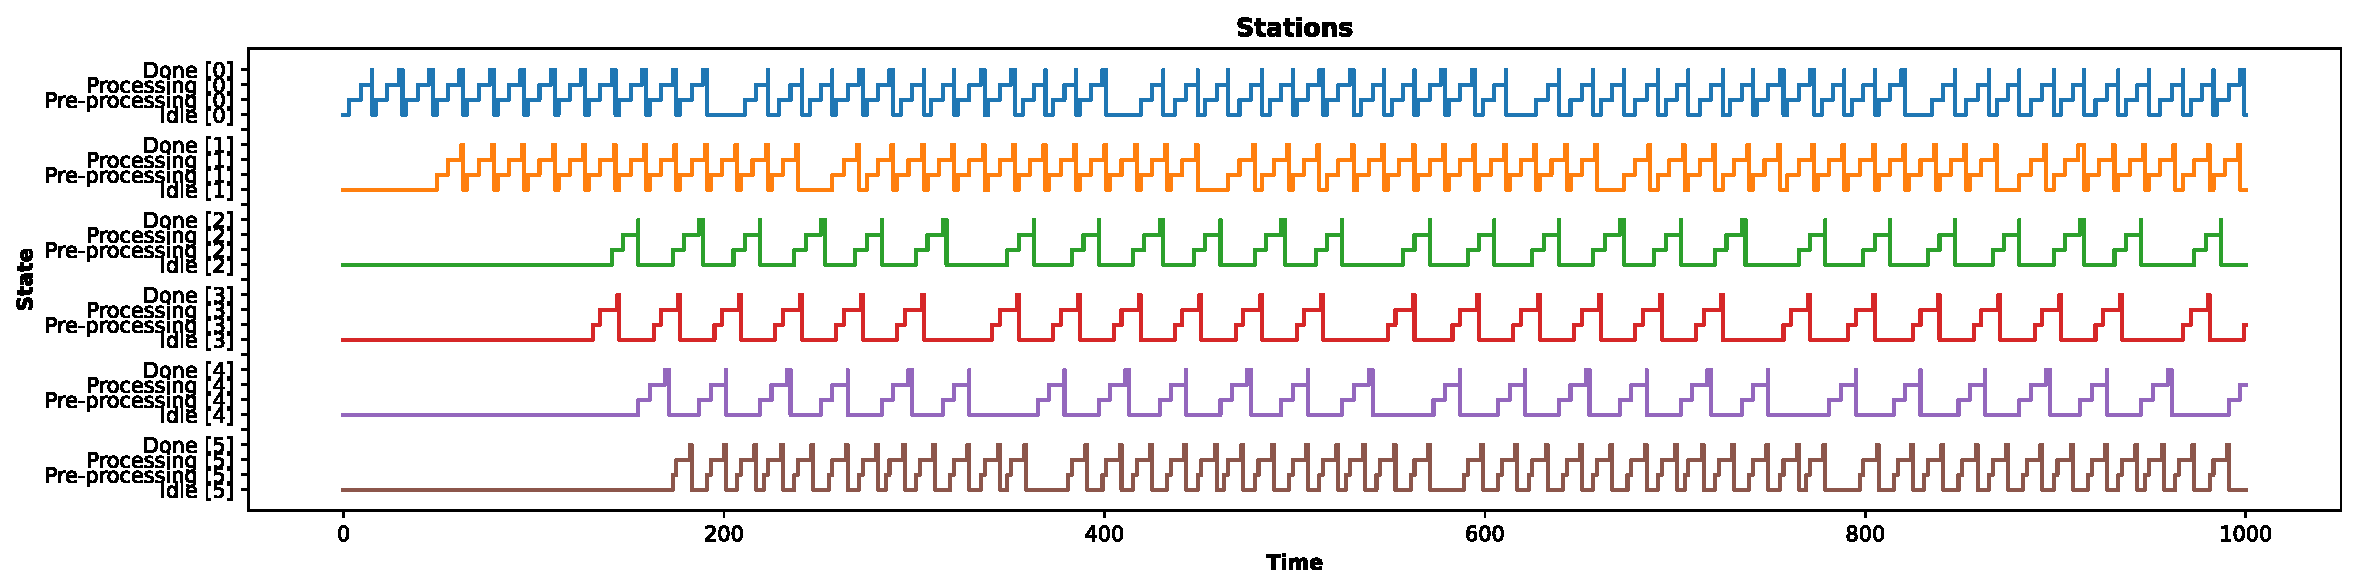
\includegraphics[width=0.9\textwidth]{images/scenarios/scenario1_stations}
        \end{subfigure}
        \begin{subfigure}{0.49\textwidth}
            \centering
            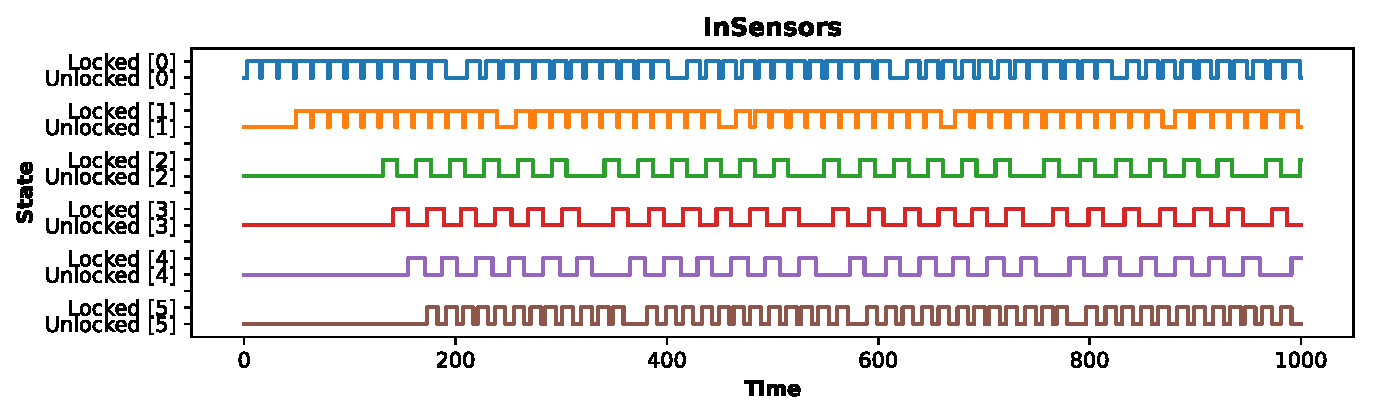
\includegraphics[width=\textwidth]{images/scenarios/scenario1_insensors}
        \end{subfigure}
        \hfill
        \begin{subfigure}{0.49\textwidth}
            \centering
            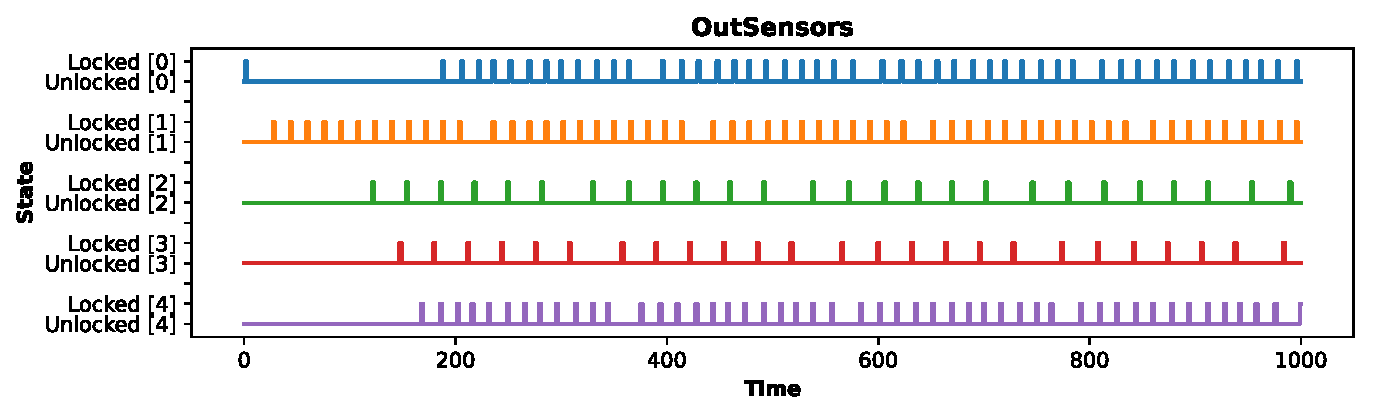
\includegraphics[width=\textwidth]{images/scenarios/scenario1_outsensors}
        \end{subfigure}
        \caption{simulation over 1000 time instants of the first scenario.}
        \label{figure:scenario:1}
    \end{figure}

    \paragraph{Results} All the properties are \textit{verified}. As it is supposed to, the plant is correctly working: every workpiece flows through the plant without any problem. The sensors are guaranteeing the required properties and the stations are working flawlessly.

    \subsection{Scenario 2: short queues}

    The idea behind this scenario is to test whether the plant is working in a realistic situation characterized by short queues of pieces waiting to be processed by the stations (i.e. each \texttt{OutSensor} is placed very close to its related \texttt{InSensor}).

    \paragraph{Parameters} These are the parameters used to obtain \figureref{figure:scenario:2}.

    \begin{center}
        \begin{tabular}{|>{\centering\arraybackslash}p{0.14\columnwidth}|>{\centering\arraybackslash}p{0.14\columnwidth}|>{\centering\arraybackslash}p{0.14\columnwidth}|>{\centering\arraybackslash}p{0.145\columnwidth}|>{\centering\arraybackslash}p{0.3\columnwidth}|}
            \hline
            \parametertt SPEED & \parametertt DISKS & \textbf{Policy} & \parametertt \small POS\_OUT\_SENSORS & \parametertt STATIONS\_ELABORATION\_TIME \\
            \hline
            1 & 12 & 3 & {\tiny [12, 33, 76, 92, 106]} & [2, 15, 5, 3, 2, 5] \\
            \hline
        \end{tabular}
    \end{center}

    \begin{figure}[h!]
        \begin{subfigure}{\textwidth}
            \centering
            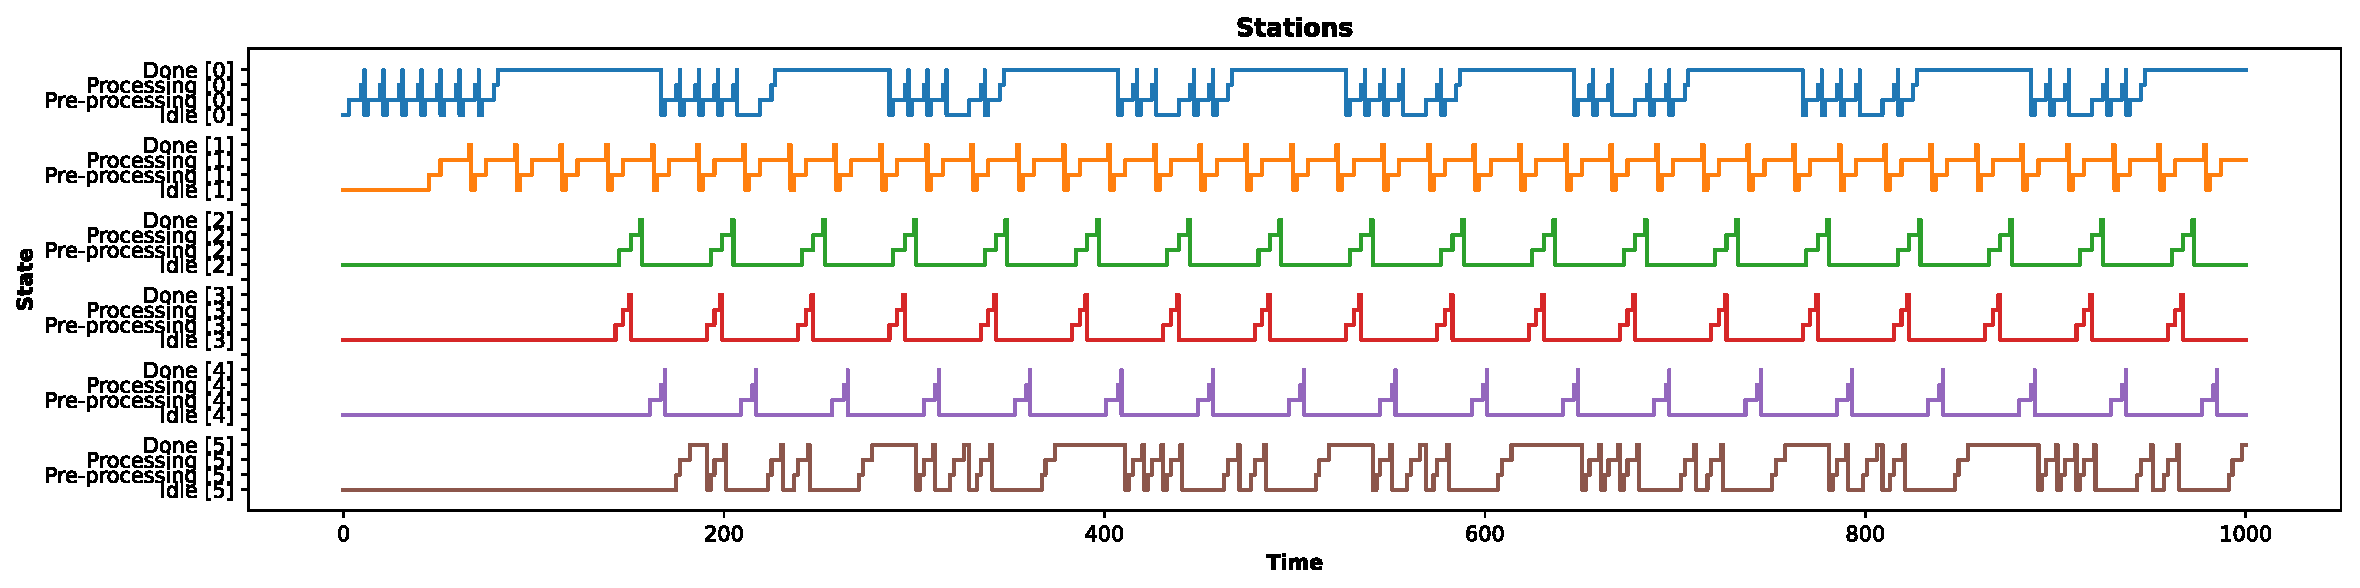
\includegraphics[width=0.9\textwidth]{images/scenarios/scenario2_stations}
        \end{subfigure}
        \begin{subfigure}{0.49\textwidth}
            \centering
            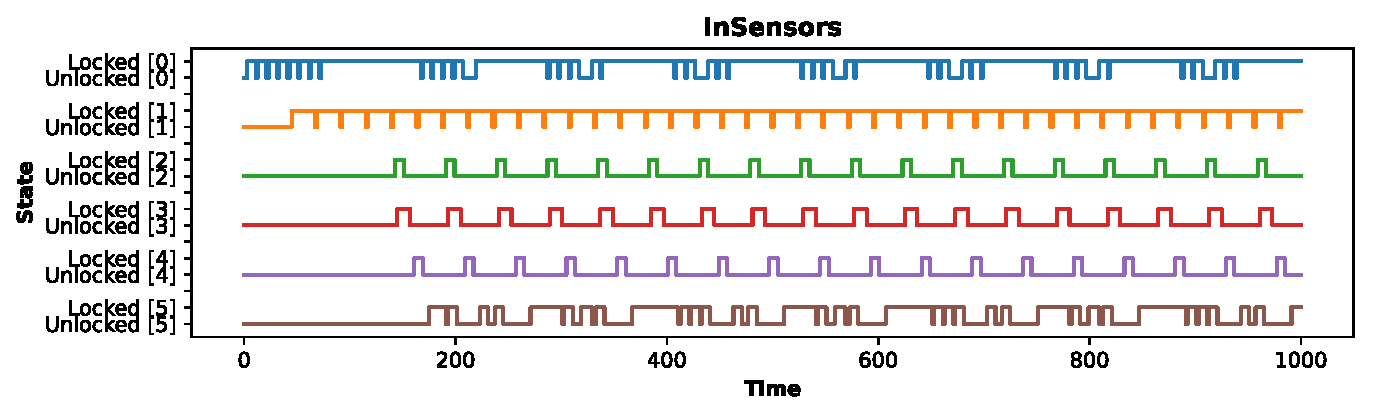
\includegraphics[width=\textwidth]{images/scenarios/scenario2_insensors}
        \end{subfigure}
        \hfill
        \begin{subfigure}{0.49\textwidth}
            \centering
            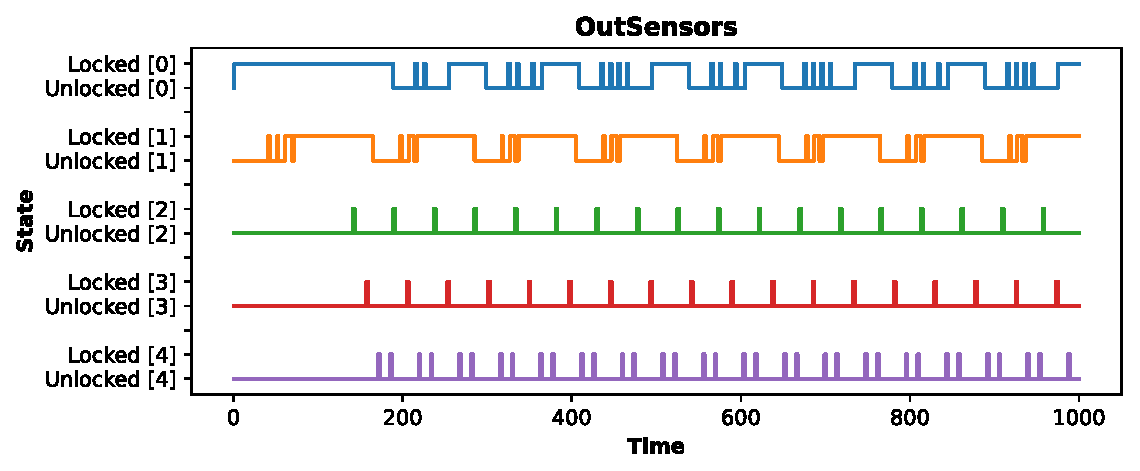
\includegraphics[width=\textwidth]{images/scenarios/scenario2_outsensors}
        \end{subfigure}
        \caption{simulation over 1000 time instants of the second scenario.}
        \label{figure:scenario:2}
    \end{figure}

    \paragraph{Results} All the properties are \textit{verified}. The graphics is showing the system is working properly without any particular delay of the stations.
    
    \paragraph{Particular case} If we slightly change the processing times of the stations (For instance by setting very short processing times on the first two stations, the same overall time on the two branches, and very long one on the last), we obtain a situation where stations 2 and 4 release a piece, which cause the saturation the queue preceding station 5, and exceeds its limit. In this case, the third property is no longer verified; anyway this behavior is completely expected, since the plant isn't smart enough to prevent this situation.

    \subsection{Scenario 3: one way}

    Here we wanted to test a different scheduling policy: we kept the same parameters of the first scenario and changed only the scheduling policy followed by the Flow Controller; in particular, we chose to route all the workpieces through the branch with the two processing stations (policy 2).

    \paragraph{Parameters} These are the parameters used to obtain \figureref{figure:scenario:3}.

    \begin{center}
        \begin{tabular}{|>{\centering\arraybackslash}p{0.14\columnwidth}|>{\centering\arraybackslash}p{0.14\columnwidth}|>{\centering\arraybackslash}p{0.14\columnwidth}|>{\centering\arraybackslash}p{0.145\columnwidth}|>{\centering\arraybackslash}p{0.3\columnwidth}|}
            \hline
            \parametertt SPEED & \parametertt DISKS & \textbf{Policy} & \parametertt \small POS\_OUT\_SENSORS & \parametertt STATIONS\_ELABORATION\_TIME \\
            \hline
            1 & 12 & 2 & {\footnotesize [2, 24, 68, 90, 105]} & [6, 7, 8, 9, 8, 7] \\
            \hline
        \end{tabular}
    \end{center}

    \begin{figure}[h!]
        \begin{subfigure}{\textwidth}
            \centering
            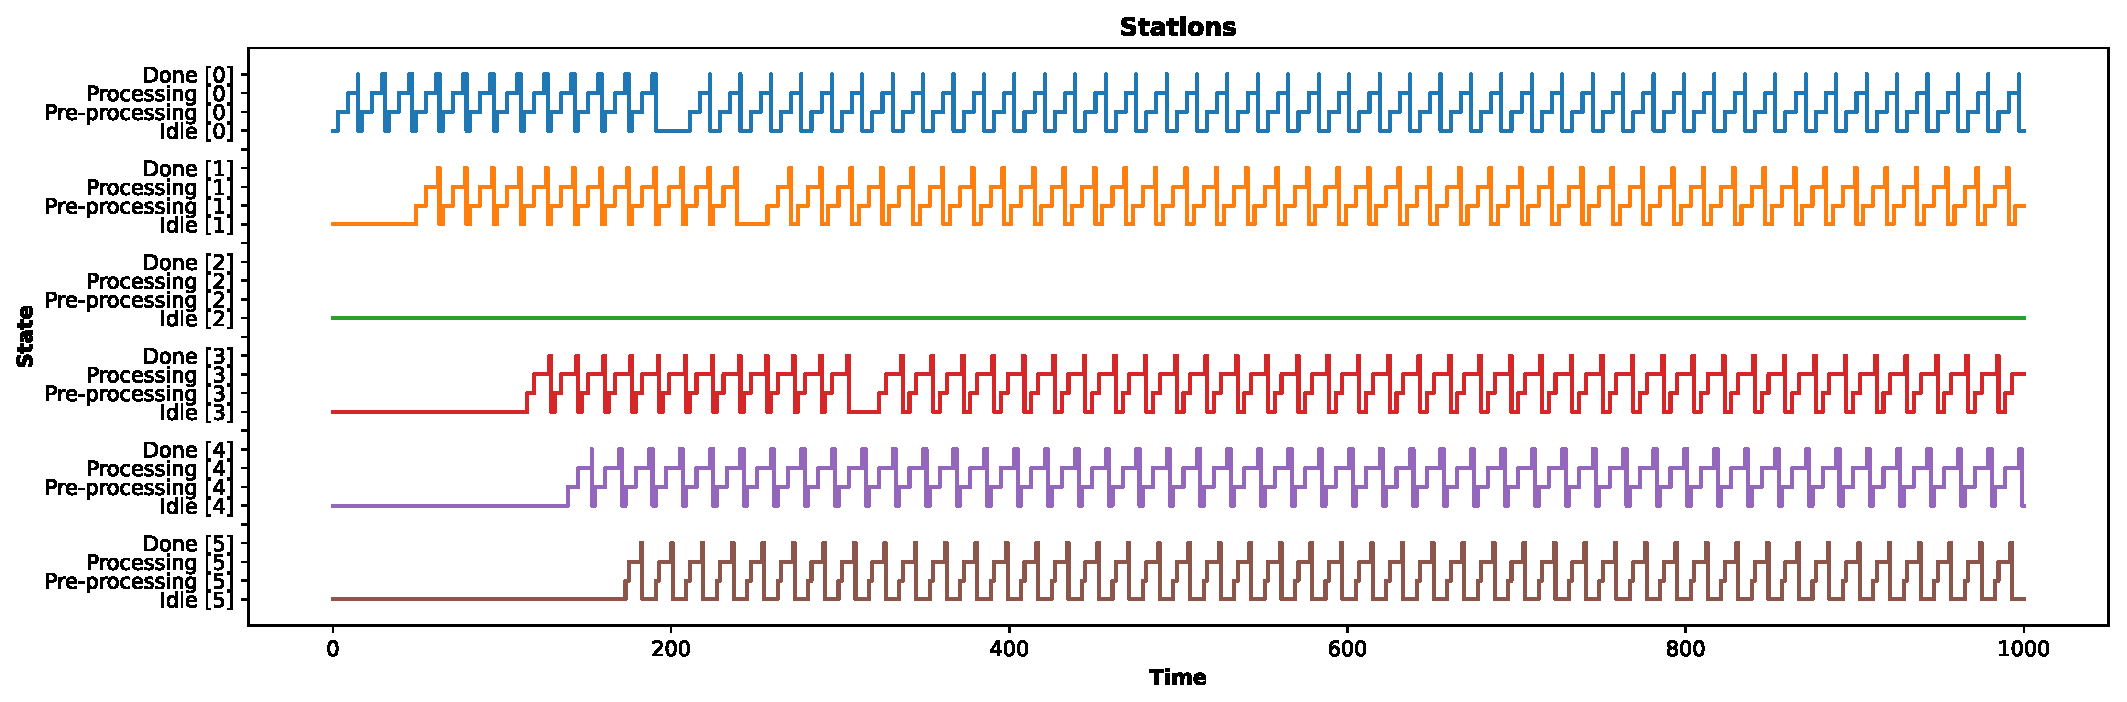
\includegraphics[width=0.9\textwidth]{images/scenarios/scenario3_stations}
        \end{subfigure}
        \begin{subfigure}{0.49\textwidth}
            \centering
            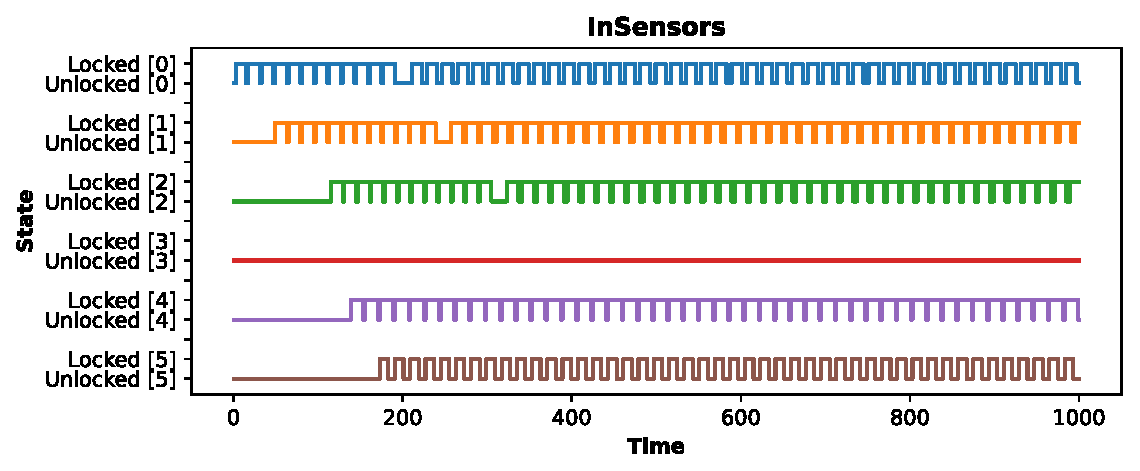
\includegraphics[width=\textwidth]{images/scenarios/scenario3_insensors}
        \end{subfigure}
        \hfill
        \begin{subfigure}{0.49\textwidth}
            \centering
            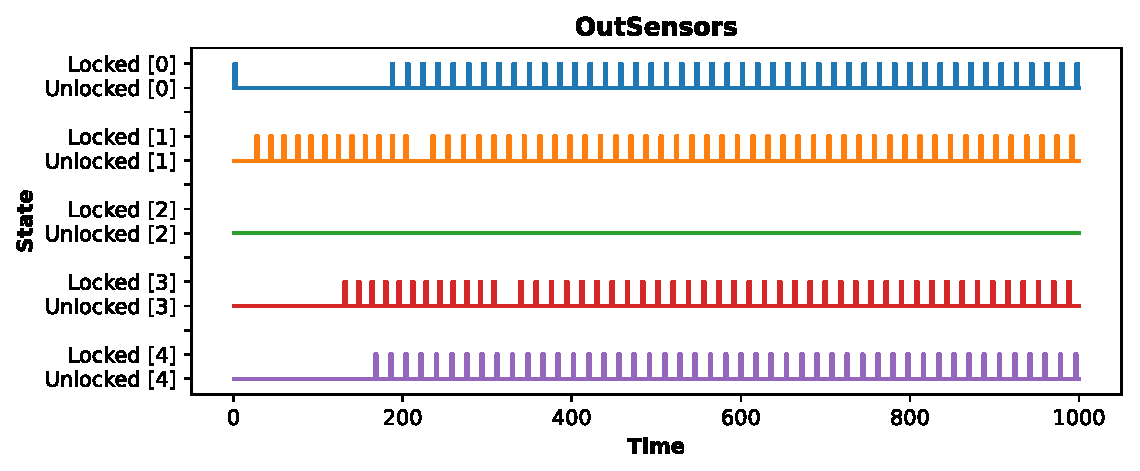
\includegraphics[width=\textwidth]{images/scenarios/scenario3_outsensors}
        \end{subfigure}
        \caption{simulation over 1000 time instants of the third scenario.}
        \label{figure:scenario:3}
    \end{figure}

    \paragraph{Results} All the properties are \textit{verified}. If we take a closer look to the graphics, we notice that the scheduling policy adopted here is slightly more inefficient w.r.t. the standard one (i.e. the one used in Scenario 1): in particular, here station 0 processes 56 pieces in 1000 time instants, while, considering the same time frame, the standard scenario is capable of processing 58 workpieces. The outcome of this comparison is easy understandable, since balancing the workload is usually the best solution.

    \subsection{Scenario 4: the stochastic case}

    Here we got the results by running the stochastic version of our project: each station's processing time varies as a Gaussian distribution around an average value, while the sensors can be faulty.

    \paragraph{Parameters} These are the parameters used to obtain \figureref{figure:scenario:4}.

    \begin{center}
        \begin{tabular}{|>{\centering\arraybackslash}p{0.14\columnwidth}|>{\centering\arraybackslash}p{0.14\columnwidth}|>{\centering\arraybackslash}p{0.14\columnwidth}|>{\centering\arraybackslash}p{0.145\columnwidth}|>{\centering\arraybackslash}p{0.3\columnwidth}|}
            \hline
            \parametertt SPEED & \parametertt DISKS & \textbf{Policy} & \parametertt \small POS\_OUT\_SENSORS & \parametertt STATIONS\_ELABORATION\_TIME \\
            \hline
            1 & 12 & 3 & {\footnotesize [2, 24, 68, 90, 105]} & [6, 7, 8, 9, 8, 7] \\
            \hline
            \hline
            \parametertitle{2}{\parametertt STD\_DEV\_STATIONS} & \parametertitle{2}{\parametertt IN\_SENSORS\_ERR} & \parametertt OUT\_SENSORS\_ERR \\
            \hline
            \parametercontent{2}{[1.0, 1.0, 1.0, 1.0, 1.0, 1.0]} & \parametercontent{2}{[1, 1, 1, 1, 1, 1]} & [1, 1, 1, 1, 1, 1] \\
            \hline
            \hline
            \parametertitle{3}{\parametertt IN\_SENSORS\_RIGHT} & \parametertitle{2}{\parametertt OUT\_SENSORS\_RIGHT} \\
            \hline
            \parametercontent{3}{[9999, 9999, 9999, 9999, 9999, 9999]} & \parametercontent{2}{[9999, 9999, 9999, 9999, 9999, 9999]} \\
            \hline
        \end{tabular}
    \end{center}

    \begin{figure}[h!]
        \begin{subfigure}{\textwidth}
            \centering
            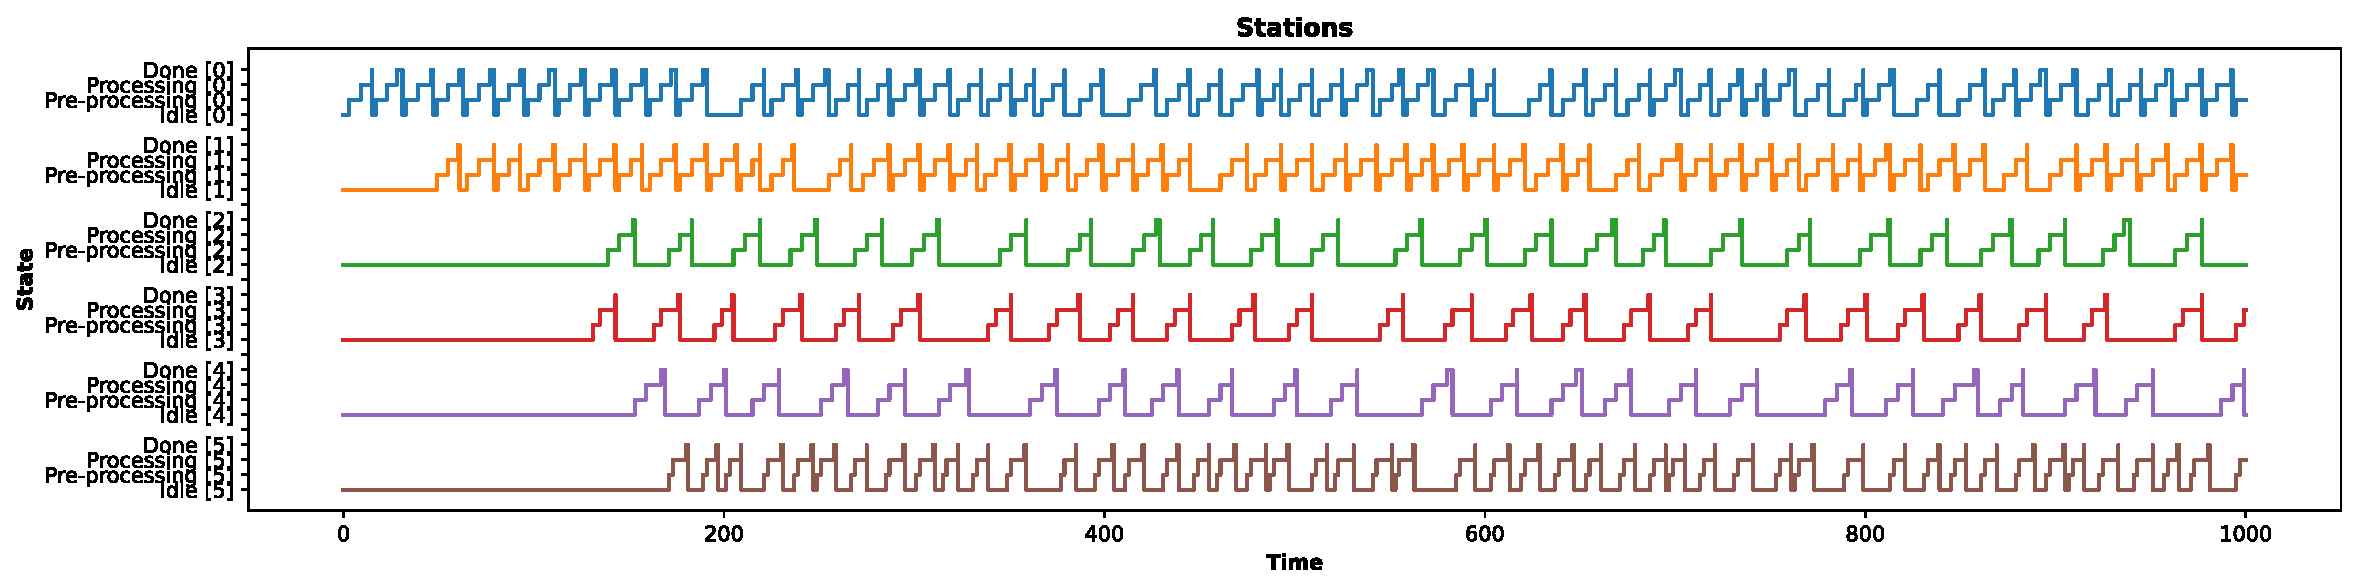
\includegraphics[width=0.9\textwidth]{images/scenarios/scenario4_stations}
        \end{subfigure}
        \begin{subfigure}{0.49\textwidth}
            \centering
            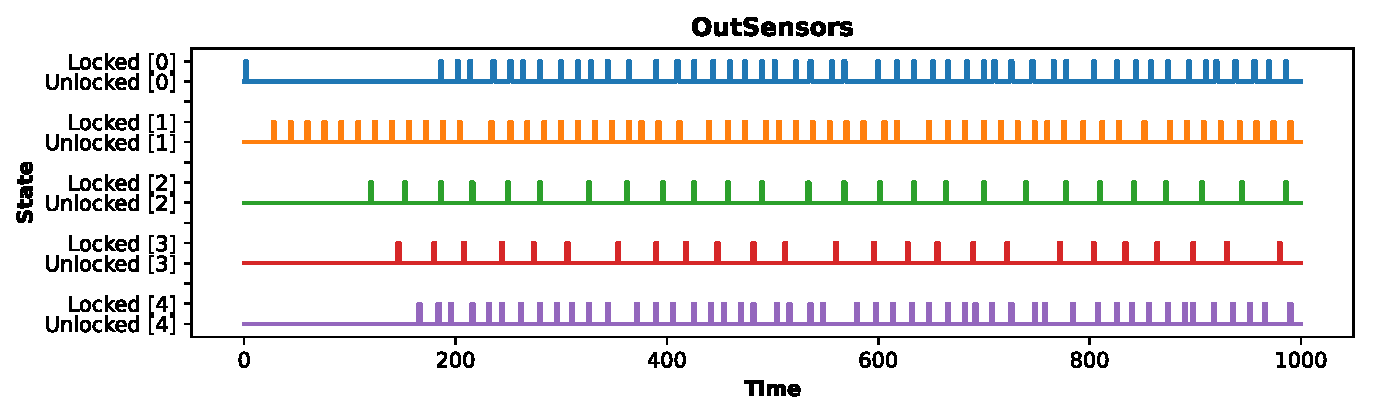
\includegraphics[width=\textwidth]{images/scenarios/scenario4_insensors}
        \end{subfigure}
        \hfill
        \begin{subfigure}{0.49\textwidth}
            \centering
            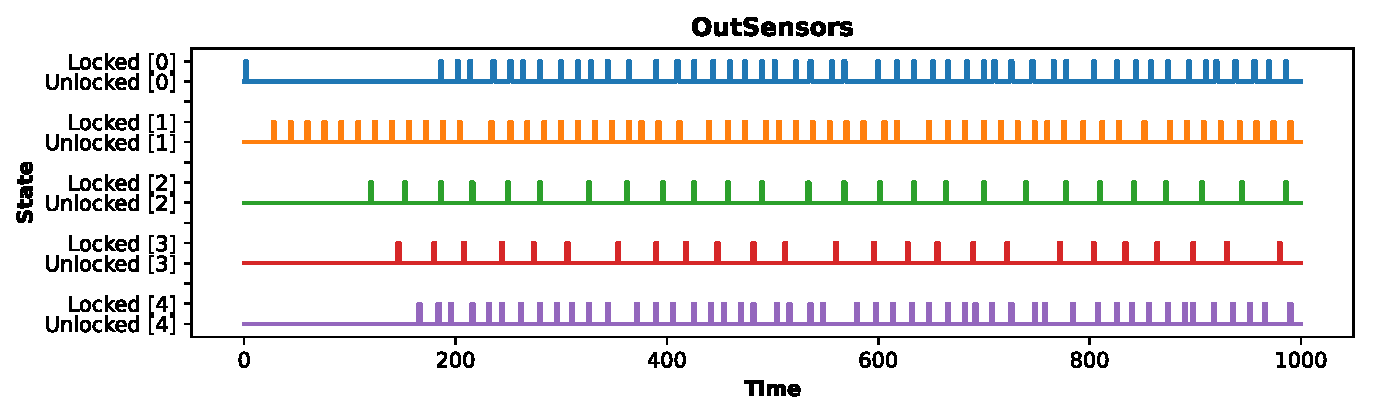
\includegraphics[width=\textwidth]{images/scenarios/scenario4_outsensors}
        \end{subfigure}
        \caption{simulation over 1000 time instants of the fourth scenario in a stochastic environment.}
        \label{figure:scenario:4}
    \end{figure}

    \paragraph{Results} All the properties are \textit{verified} with a 95\% confidence and with the following probabilities:
    \begin{itemize}
        \item \(> 95\%\) (\propertyref{1}{property:1-2});
        \item \(84\% \pm 5\%\) (\propertyref{2}{property:3});
        \item \(> 95\%\) (\propertyref{3}{property:4}).
    \end{itemize}
    We can see that the plant is still working in a non-ideal scenario, correctly processing all the workpieces, without breaking physics constraints. Note that it may happen that some queues exceeds their maximum length, because of faulty sensors.

    \subsection{Scenario 5: the faulty stochastic}

    The goal here is to show that in the (unrealistic) case of a stochastic production plant with highly faulty sensors, the system keeps working properly, even if the queues maximum lengths can't be guaranteed.

    \paragraph{Parameters} These are the parameters used to obtain \figureref{figure:scenario:5}.

    \begin{center}
        \begin{tabular}{|>{\centering\arraybackslash}p{0.14\columnwidth}|>{\centering\arraybackslash}p{0.14\columnwidth}|>{\centering\arraybackslash}p{0.14\columnwidth}|>{\centering\arraybackslash}p{0.145\columnwidth}|>{\centering\arraybackslash}p{0.3\columnwidth}|}
            \hline
            \parametertt SPEED & \parametertt DISKS & \textbf{Policy} & \parametertt \small POS\_OUT\_SENSORS & \parametertt STATIONS\_ELABORATION\_TIME \\
            \hline
            1 & 12 & 3 & {\footnotesize [2, 24, 68, 90, 105]} & [6, 7, 8, 9, 8, 7] \\
            \hline
            \hline
            \parametertitle{2}{\parametertt STD\_DEV\_STATIONS} & \parametertitle{2}{\parametertt IN\_SENSORS\_ERR} & \parametertt OUT\_SENSORS\_ERR \\
            \hline
            \parametercontent{2}{[1.0, 1.0, 1.0, 1.0, 1.0, 1.0]} & \parametercontent{2}{[1, 1, 1, 1, 1, 1]} & [1, 1, 1, 1, 1, 1] \\
            \hline
            \hline
            \parametertitle{3}{\parametertt IN\_SENSORS\_RIGHT} & \parametertitle{2}{\parametertt OUT\_SENSORS\_RIGHT} \\
            \hline
            \parametercontent{3}{[99, 99, 99, 99, 99, 99]} & \parametercontent{2}{[99, 99, 99, 99, 99, 99]} \\
            \hline
        \end{tabular}
    \end{center}

    \begin{figure}[h!]
        \begin{subfigure}{\textwidth}
            \centering
            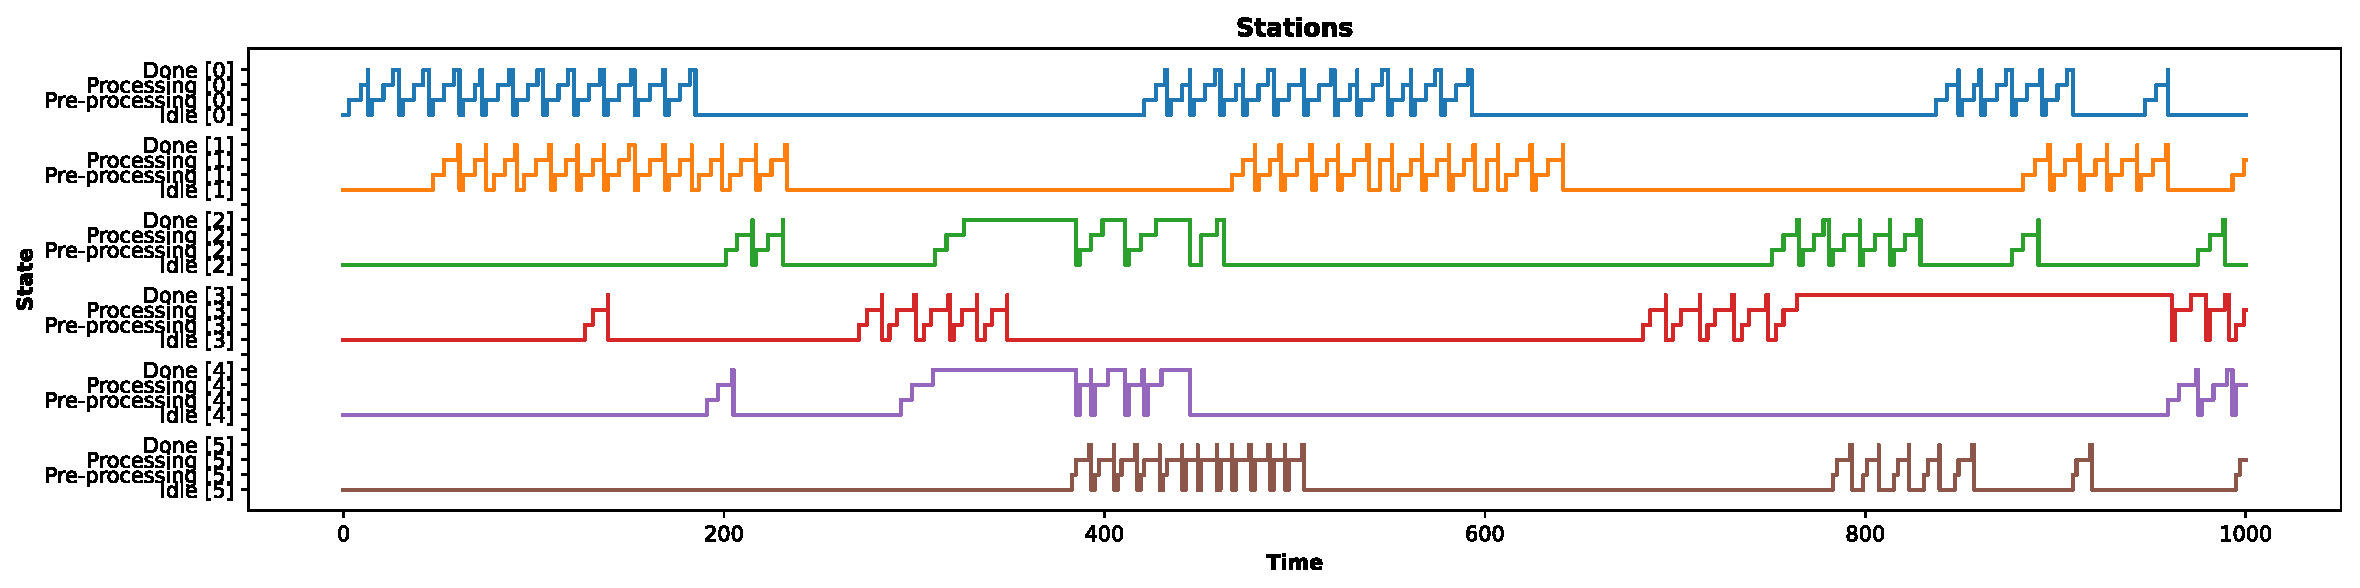
\includegraphics[width=0.9\textwidth]{images/scenarios/scenario5_stations}
        \end{subfigure}
        \begin{subfigure}{0.49\textwidth}
            \centering
            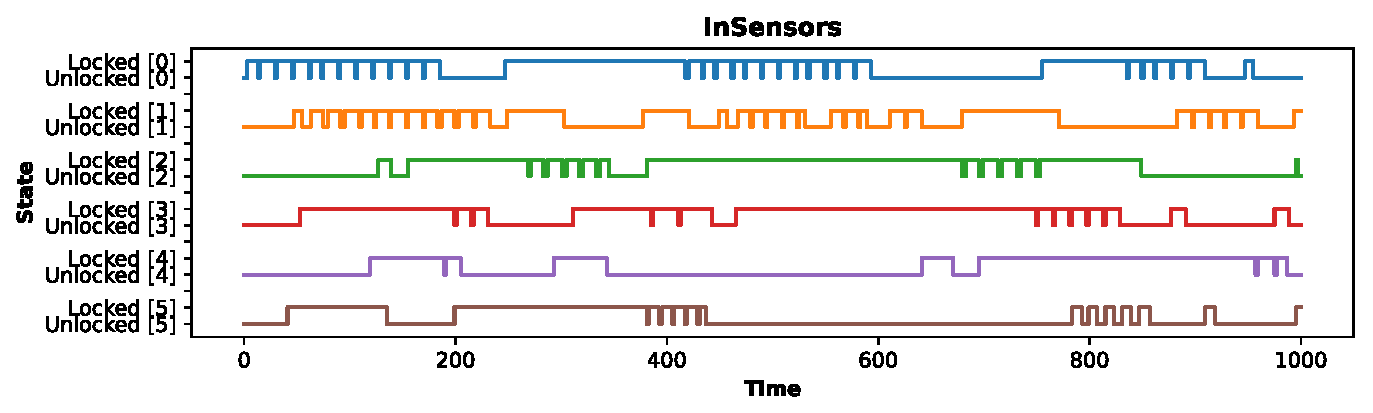
\includegraphics[width=\textwidth]{images/scenarios/scenario5_insensors}
        \end{subfigure}
        \hfill
        \begin{subfigure}{0.49\textwidth}
            \centering
            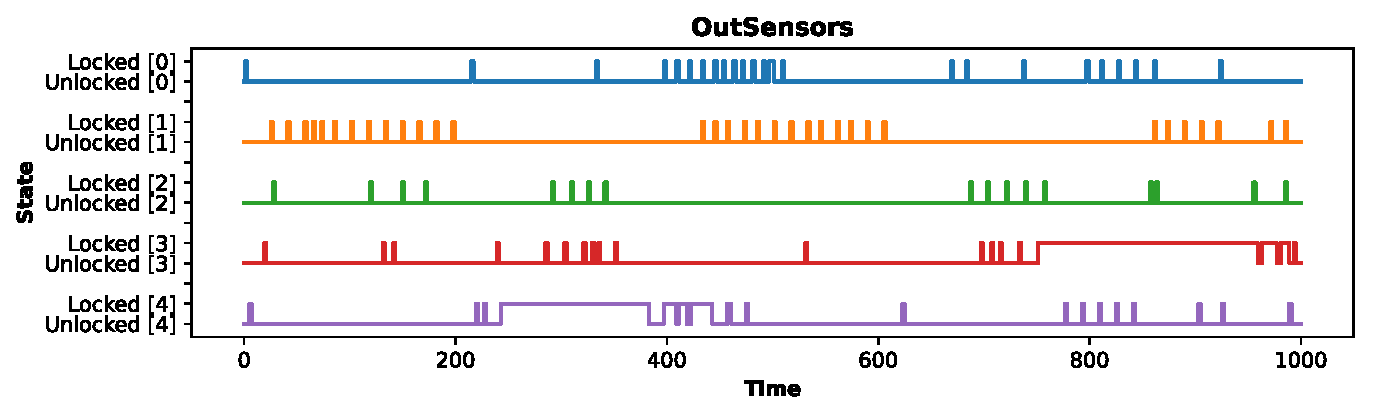
\includegraphics[width=\textwidth]{images/scenarios/scenario5_outsensors}
        \end{subfigure}
        \caption{simulation over 1000 time instants of the fifth scenario in a stochastic environment.}
        \label{figure:scenario:5}
    \end{figure}

    \paragraph{Results} Some properties are \textit{not verified}, but all with a 95\% confidence; we achieved the following probabilities:
    \begin{itemize}
        \item \(> 95\%\) (\propertyref{1}{property:1-2});
        \item \(< 5\%\) (\propertyref{2}{property:3});
        \item \(> 95\%\) (\propertyref{3}{property:4}).
    \end{itemize}
    It is clear that, also in this case, the plant is still functioning, even if it's almost certain that at least one queue exceed its maximum length. This is due to the very high probability of a sensor to be faulty, for which in 10000 time instants, this property can't be fully verified. However, the plant doesn't incur in any deadlock and physical constraints are respected.

    \section{Conclusions}

    In conclusion, we argue that the results obtained in the various scenarios just presented can be considered proofs of the efficiency and the resiliency achieved by the proposed model. We can state that our project provides a complete abstraction of the LEGO® MINDSTROMS™ Production Plant, by considering both common and rare situations, without neglecting any corner case. From the perspective of performance, we think that, after several optimizations and refinements, we have achieved remarkable outcomes, both in terms of verification speed and memory consumption. By virtue of the considerations exhibited so far, we deeply believe that our model is sticking close to the specifications required by the LEGO® MINDSTROMS™ Production Plant's model.

\end{document}
